\chapter{DISEÑO DE LA ETAPA DE CONTROL}\label{cap:control}
\listasdecapitulo{6}

\section{Arquitectura de control en tres capas}\label{sec:arquitectura-control}

El módulo de control propuesto para la red semafórica de Lima Metropolitana busca superar
las limitaciones de los sistemas de tiempo fijo y programable que operan en la mayoría de
intersecciones de la ciudad, los cuales no responden a las condiciones reales del tráfico y
generan tiempos de espera excesivos, congestión crónica y desperdicio de capacidad vial en
periodos de baja demanda. Frente a ello, el diseño no reemplaza al controlador semafórico
existente, sino que añade una capa de sensado y decisión que \emph{recomienda} ajustes de
fase. La premisa arquitectónica, sostenida en todo el documento, es que el controlador
semafórico conserva la autoridad final de actuación y que ninguna salida del módulo se
convierte por sí sola en una orden de lámpara.

El sistema integra tres capas que operan de forma sinérgica y en escalas temporales
complementarias:

\begin{enumerate}
\item \textbf{Capa de percepción.} Una cámara domo de visión cenital (modelo
  DS-2CE57H0T-VPITF) instalada en el centro de cada intersección $I_{p}$ captura video que,
  procesado mediante detección de objetos (YOLO) y seguimiento (ByteTrack), produce las
  variables locales de tráfico: cola, velocidad, flujo, densidad y presencia de vehículos de
  emergencia.
\item \textbf{Capa de decisión local (núcleo validable).} Un controlador difuso de Mamdani,
  ejecutado en el cómputo de borde de la intersección, integra esas variables en el Índice de
  Congestión Vehicular (ICV) y genera un ajuste acotado del tiempo verde. Opera con latencia
  baja, es interpretable y sobrevive a la pérdida de conectividad. Constituye el núcleo
  validable del módulo.
\item \textbf{Capa de coordinación global (soporte no crítico).} Una infraestructura en la
  nube (Microsoft Azure) recibe la telemetría de todas las intersecciones, calcula métricas de
  red y coordinación entre cruces y emite recomendaciones globales. Esta capa es de soporte:
  su indisponibilidad degrada el desempeño de coordinación, pero no impide que la capa local
  continúe operando con su plan seguro.
\end{enumerate}

La lógica difusa se selecciona como núcleo porque ofrece reglas interpretables, incorpora
conocimiento experto, opera con pocos datos iniciales, se ejecuta en el borde y permite
verificar sistemáticamente sus límites. Las capas de aprendizaje por refuerzo (RL) y de
predicción CNN--LSTM se presentan como módulos experimentales de optimización y extensión
futura (Sección~\ref{sec:capas-futuras}), no como sustitutos del controlador certificado.
Esta delimitación mantiene la propuesta dentro de un alcance técnico realista para una tesis
de titulación.

\section{Percepción y variables locales}\label{sec:percepcion}

La capa de percepción opera de manera autónoma en cada intersección $I_{p}$, procesando en
tiempo real el video de la cámara domo para extraer las variables que alimentan la decisión
local. Todas las variables se calculan por dirección y se organizan en vectores que se
actualizan según la orientación de la cámara.

\subsection{Orientación de cámara y función de máscara}\label{subsec:cammask}

La cámara domo alterna entre dos vistas perpendiculares para cubrir los cuatro accesos de la
intersección cruciforme: la vista Norte--Sur (NS), que observa los carriles Norte y Sur, y la
vista Este--Oeste (EO), que observa los carriles Este y Oeste. El estado de observación en el
instante $t$ se representa mediante la función de máscara:
\[
CamMask(I_{p},t) =
\begin{cases}
1, & \text{si la cámara apunta hacia Norte--Sur}\\[2pt]
0, & \text{si la cámara apunta hacia Este--Oeste}
\end{cases}
\]

Esta función determina qué grupo de carriles (NS o EO) está visible para el cálculo de
métricas en un instante dado y controla la actualización de los vectores de estado local.

\subsection{Política de orientación y actualización confiable de variables}\label{subsec:politica-orientacion}

La función de máscara de cámara no solo identifica qué eje se encuentra visible, sino que también
gobierna la validez temporal de las variables estimadas. Para evitar que el movimiento de la cámara
introduzca mediciones inestables, el proceso de observación se divide en tres estados:
\emph{movimiento}, \emph{estabilización} y \emph{observación válida}.

En el estado \textit{MOVING} la cámara transita hacia la orientación objetivo; durante ese intervalo
los cuadros no se emplean para actualizar el ICV ni las variables locales, por la posible presencia de
desenfoque, vibración o pérdida parcial de las regiones de interés. En el estado \textit{SETTLING} la
cámara ya alcanzó la posición objetivo, pero se respeta una breve ventana de estabilización antes de
aceptar nuevas mediciones. Finalmente, en el estado \textit{OBSERVING} la inferencia visual se
considera válida siempre que se cumplan los umbrales mínimos de confianza del detector y las variables
estimadas permanezcan dentro de rangos físicos plausibles.

La actualización de los vectores de estado local se realiza únicamente en el estado \textit{OBSERVING}.
Durante \textit{MOVING} y \textit{SETTLING}, el módulo conserva el último vector válido de cada eje
junto con su marca temporal; si la antigüedad de ese vector supera un umbral máximo de vigencia, la
información se declara no confiable para control adaptativo y el sistema pasa a un modo conservador o
degradado. Formalmente, el vector de estado de cada eje $d$ se actualiza según:
\[
X_d(t)=
\begin{cases}
\hat{X}_d(t), & \text{si } CamState(t)=\textit{OBSERVING}\ \wedge\ Conf(t)\geq \tau_{det},\\[2pt]
X_d(t^{-}), & \text{si } CamState(t)\in\{\textit{MOVING},\textit{SETTLING}\}\ \wedge\ t-t_{last,d}\leq T_{valid},\\[2pt]
\varnothing, & \text{si } t-t_{last,d}>T_{valid},
\end{cases}
\]
donde $\hat{X}_d(t)$ es el vector estimado por visión, $Conf(t)$ la confianza agregada de detección,
$\tau_{det}$ el umbral mínimo de confianza, $t_{last,d}$ el instante de la última actualización válida
y $T_{valid}$ el tiempo máximo permitido para reutilizar una estimación previa. El caso $\varnothing$
(sin dato vigente) activa el modo degradado descrito en la Sección~\ref{sec:modos-operacion}.

Esta política evita que una detección puntual, un cuadro borroso o una medición obtenida durante la
reorientación de la cámara modifiquen directamente la recomendación del controlador difuso. Además, el
ICV se calcula a partir de variables agregadas en ventanas temporales y no desde una única detección
instantánea, lo que añade robustez frente a errores transitorios de percepción.

\subsection{Funciones de detección}\label{subsec:funciones-deteccion}

\textbf{Cola vehicular (conteo de detenidos).} Cuantifica los vehículos prácticamente
inmóviles en cada carril, indicador directo de demanda acumulada:
\[
StoppedCount(l,t) = \sum_{v \in V(l,t)}\delta[v],
\qquad
\delta[v] =
\begin{cases}
1, & \text{si } velocidad(v) < \varepsilon\\[2pt]
0, & \text{caso contrario}
\end{cases}
\]
donde $V(l,t)$ es el conjunto de vehículos detectados en el carril $l$, $velocidad(v)$ la
velocidad instantánea estimada por ByteTrack y $\varepsilon$ el umbral para considerar un
vehículo detenido.

\textbf{Velocidad promedio.} Evalúa la fluidez considerando solo vehículos en movimiento:
\[
V_{avg}(l,t) = \frac{1}{N_{mov}(l,t)}\sum_{v \in V_{mov}(l,t)}velocidad(v),
\qquad
V_{mov}(l,t) = \{ v \in V(l,t): velocidad(v) \geq \varepsilon\}.
\]
Para que la variable quede definida en todo escenario se adoptan dos convenciones de borde: si
no hay vehículos en el carril ($N_{total}=0$) se asigna $V_{avg}=V_{MAX}$, pues la ausencia de
demanda equivale a flujo libre; si hay vehículos pero todos están detenidos
($N_{total}>0 \land N_{mov}=0$) se asigna $V_{avg}=0$, el caso de máxima retención. Estas
convenciones evitan indeterminaciones del promedio y garantizan que los índices derivados
interpreten correctamente tanto la vía vacía como la bloqueada.

\textbf{Flujo vehicular.} Mide la tasa de salida de vehículos, útil para estimar capacidad y
eficiencia instantánea:
\[
q(l,t) = \frac{N_{cross}(l,\ t_{0},\ t)}{t-t_{0}},
\]
donde $N_{cross}$ es el número de vehículos que cruzaron una línea de conteo virtual entre los
tiempos $t_{0}$ y $t$.

\textbf{Densidad vehicular.} Refleja la ocupación espacial del carril:
\[
k(l,t) = \frac{N_{total}(l,t)}{L_{efectiva}},
\qquad N_{total}(l,t)=|V(l,t)|.
\]
A diferencia del modelo clásico $k=q/V_{avg}$, esta formulación calcula la densidad
espacialmente contando directamente los vehículos en un área conocida, lo cual resulta más
adecuado para sistemas de visión por computadora.

\textbf{Detección de vehículos de emergencia (capacidad habilitada por la arquitectura).} Se contempla
la identificación de ambulancias y vehículos de bomberos para activar políticas de priorización; en el
presente alcance constituye una \emph{entrada prioritaria de diseño}, no una función validada
experimentalmente:
\[
EV(l,t) = \sum_{v \in V(l,t)}\delta_{emg}[v,t],
\qquad
\delta_{emg}[v,t] =
\begin{cases}
1, & \text{si } class(v)\in C_{emg}\ \land\ confidence(v)\geq \tau_{EV}\\[2pt]
0, & \text{caso contrario}
\end{cases}
\]
donde $C_{emg}=\{\text{ambulancias, bomberos}\}$ y $\tau_{EV}=0.85$ es el umbral mínimo de
confianza, fijado alto para minimizar falsos positivos dado el fuerte impacto de una
activación errónea de prioridad. Una vez detectado un vehículo de emergencia, ByteTrack lo
sigue de forma continua registrando posición, velocidad y direcciones de entrada y salida, e
incluso reorienta la cámara de forma reactiva (mediante zonas de activación calibradas en el
plano de la intersección) para no perder su visibilidad al girar dentro del cruce. La detección
\emph{confiable} de vehículos de emergencia —mediante visión entrenada, señal acústica o mensajería
V2X— excede el alcance de esta tesis y se documenta como extensión futura
(Sección~\ref{sec:capas-futuras}).

Todas las variables se vectorizan según la orientación de cámara; por ejemplo, para la cola:
\[
SC_{p}(t) =
\begin{cases}
\left[\, SC_{N},\ SC_{S},\ 0,\ 0 \,\right], & CamMask(I_{p},t) = 1\\[2pt]
\left[\, 0,\ 0,\ SC_{E},\ SC_{O} \,\right], & CamMask(I_{p},t) = 0
\end{cases}
\]
con expresiones análogas para $V_{avg}$, $q$, $k$ y $EV$. En cada instante solo dos
direcciones reciben valores observados; las dos restantes conservan su última lectura válida.

\subsection{Parámetro de Intensidad (PI)}\label{subsec:pi}

El Parámetro de Intensidad cuantifica la relación entre fluidez (velocidad) y acumulación
(cola), permitiendo detectar estados de congestión inminente donde la velocidad cae mientras
la cola crece:
\[
PI(l,t) = \frac{V_{avg}(l,t)+\delta}{SC(l,t)+\delta},
\]
con $\delta=0.1$ una pequeña constante de regularización que evita la división entre cero. Como
$V_{avg}$ y $SC$ ingresan normalizados a $[0,1]$, el cociente crudo es asimétrico, por lo que
el indicador se acota mediante la transformación racional:
\[
PI_{norm}(l,t) = \frac{PI(l,t)}{1+PI(l,t)}
= \frac{V_{avg}(l,t)+\delta}{V_{avg}(l,t)+SC(l,t)+2\delta}.
\]
Esta transformación es estrictamente creciente y reparte el rango de salida de forma
equilibrada: cuando velocidad y cola se igualan resulta $PI_{norm}=0.5$ (equilibrio entre
movilidad y retención); el flujo libre puro produce $PI_{norm}\approx 0.92$ y el bloqueo total
$PI_{norm}\approx 0.08$. Esta propiedad da significado físico directo a los umbrales de los
conjuntos difusos definidos más adelante. En adelante, toda referencia al PI alude a
$PI_{norm}$.

\subsection{Matriz de estado local y transmisión}\label{subsec:matriz-estado}

Las variables anteriores, más el ICV y el PI por dirección, se consolidan en la matriz de
estado local de la intersección, de dimensión $\mathbb{R}^{28}$ (7 variables $\times$ 4
direcciones):
\[
X_{\text{local}}^{(p)}(t)=
\big[\,SC_{d},\ V_{avg,d},\ q_{d},\ k_{d},\ ICV_{d},\ PI_{d},\ EV_{d}\,\big]_{d\in\{N,S,E,O\}}
\in \mathbb{R}^{28}.
\]
La normalización se aplica \emph{por variable} y no sobre el vector completo,
$X_{norm}=(X-X_{MIN})/(X_{MAX}-X_{MIN})$, empleando matrices auxiliares $X_{MAX}$ y $X_{MIN}$
reconfigurables. Un único rango global mezclaría escalas heterogéneas y anularía las variables
de menor magnitud (como las banderas de emergencia). El vector resultante se transmite al
servicio en la nube mediante un paquete de telemetría que incluye identificador de
intersección, marca temporal UTC, fase actual, tiempo restante, estado de conexión y un hash
SHA-256 de integridad; cuando $EV_{d}>0$ se activa un canal de transmisión prioritario con el
estado cinemático del vehículo de emergencia. La relación entre las funciones de detección y
los índices integrados se ilustra en la Figura~\ref{fig:variables-locales} y su consolidación
en la matriz de estado en la Figura~\ref{fig:matriz-estado}.

\begin{figure}[H]
  \centering
  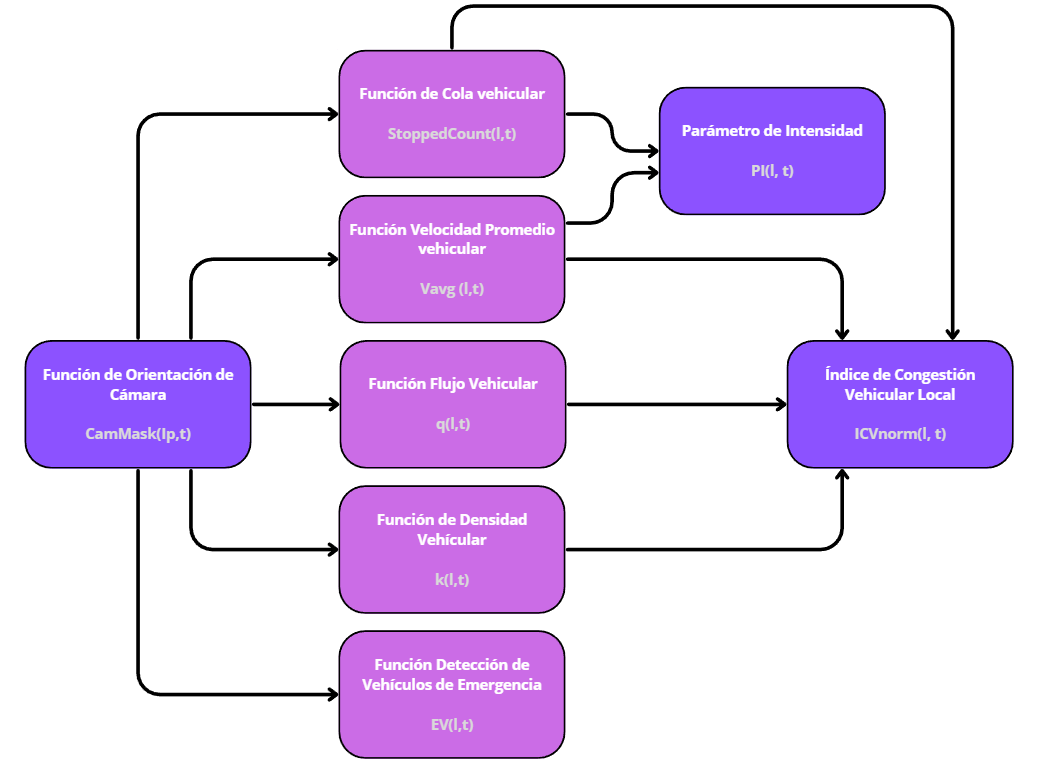
\includegraphics[width=0.9\linewidth,keepaspectratio]{media/image95.png}
  \caption{Relación de las variables locales: las cinco funciones de detección alimentan los
  índices integrados PI e ICV de cada carril.}
  \label{fig:variables-locales}
  \fuente{Elaboración propia.}
\end{figure}

\begin{figure}[H]
  \centering
  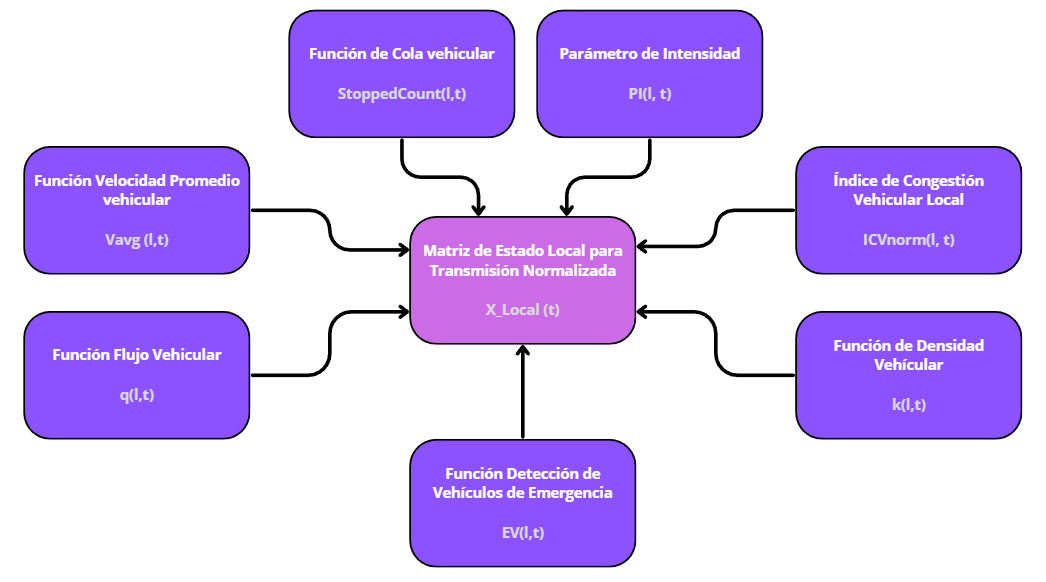
\includegraphics[width=0.9\linewidth,keepaspectratio]{media/image143.png}
  \caption{Relación de las variables locales con la matriz de estado local transmitida a la nube.}
  \label{fig:matriz-estado}
  \fuente{Elaboración propia.}
\end{figure}

\section{Índice de Congestión Vehicular (ICV)}\label{sec:icv}

El ICV integra las variables de tráfico en un índice sintético continuo, normalizado en
$[0,1]$, que representa el nivel de congestión de cada carril. Constituye la entrada compuesta
principal del controlador difuso y, por su interpretabilidad, la base de la visualización de
estado para los operadores.

\subsection{Formulación y compuerta por demanda}\label{subsec:icv-formula}

\[
ICV(l,t) =
\begin{cases}
0, & \text{si } N_{total}(l,t)=0\\[6pt]
w_{1}\dfrac{SC(l,t)}{SC_{MAX}}
+ w_{2}\!\left(1-\dfrac{V_{avg}(l,t)}{V_{MAX}}\right)
+ w_{3}\dfrac{q(l,t)}{q_{MAX}}
+ w_{4}\dfrac{k(l,t)}{k_{MAX}}, & \text{si } N_{total}(l,t)>0
\end{cases}
\]

En esta formulación $q_{MAX}$ es el flujo de saturación del acceso, de modo que el término
$q/q_{MAX}$ es el \emph{grado de saturación} (razón volumen--capacidad), un indicador clásico de
congestión en ingeniería de tránsito: cuanto más se aproxima el flujo servido a la capacidad del
acceso, mayor es la presión de demanda y el término crece hacia $1$. Así, los cuatro sumandos
aumentan de forma coherente con la congestión ---cola detenida, retención de velocidad, grado de
saturación y ocupación espacial---, tal como confirman los casos de prueba de la
Sección~\ref{subsec:icv-casos} y el análisis de sensibilidad de la
Sección~\ref{subsec:icv-sensibilidad}, donde un aumento del flujo eleva el ICV. La compuerta por
demanda ($ICV=0$ cuando no hay vehículos) resuelve la ambigüedad del flujo bajo: una vía vacía y
una vía bloqueada producen ambas $q\approx 0$, pero solo la segunda está congestionada; al
condicionar el índice a la presencia de vehículos detectados, la vía vacía no registra congestión,
mientras que la vía bloqueada queda correctamente capturada por los términos de cola, velocidad y
densidad. La restricción de convexidad $\sum_{i=1}^{4}w_{i}=1$, $w_{i}\geq 0$, garantiza que el
ICV sea una combinación convexa de términos acotados en $[0,1]$ y, por lo tanto, quede acotado en
$[0,1]$ sin reescalamiento posterior.

\subsection{Pesos, verificación por AHP y parámetros}\label{subsec:icv-pesos}

Los pesos se asignan por ponderación directa a partir del criterio del autor, fundamentado en la
literatura de ingeniería de tránsito, priorizando la cola detenida como el indicador más directo
de demanda insatisfecha: $w_{1}=0.35$ (cola), $w_{2}=0.25$ (velocidad), $w_{3}=0.25$ (flujo) y
$w_{4}=0.15$ (densidad). Esta asignación se verifica de forma independiente mediante el método de
jerarquías analíticas (AHP). La matriz de comparación por pares (Tabla~\ref{tab:ahp}) se construye
con la escala de Saaty a partir de los mismos juicios relativos: la cola se considera moderadamente
más importante que la velocidad y el flujo (razón $1.5$) y claramente más importante que la densidad
(razón $2.5$). El vector propio principal arroja los pesos normalizados
$(0.362,\,0.253,\,0.253,\,0.132)$, que coinciden en orden y magnitud con la ponderación directa. La
consistencia de los juicios se confirma con $\lambda_{\max}=4.004$, índice de consistencia
$\mathrm{IC}=0.001$ y \textbf{razón de consistencia} $\mathrm{RC}=0.002$, muy por debajo del umbral
de $0.1$ recomendado por Saaty. El refinamiento adicional de estos pesos mediante una búsqueda de
optimización —por ejemplo, un barrido sobre el simplex $\sum w_{i}=1$ en SUMO que minimice la demora
media— no se ejecuta en esta tesis y se plantea como trabajo futuro; los resultados de validación del
Capítulo~\ref{cap:validacion} no dependen de dicho ajuste, pues emplean los pesos aquí justificados.
Conviene precisar, además, que el ICV es la \emph{entrada} compuesta del controlador y no la métrica
de éxito de la validación: esta se sustenta en la demora, la cola, el \textit{throughput} y la
velocidad de red.

\begin{table}[H]
  \centering
  \caption{Matriz de comparación por pares (escala de Saaty) y verificación de los pesos del ICV.}
  \label{tab:ahp}
  \begin{tabular}{@{}lcccccc@{}}
    \toprule
    \textbf{Criterio} & \textbf{L} & \textbf{V} & \textbf{F} & \textbf{D} & \textbf{Peso AHP} & \textbf{Pond.\ directa} \\
    \midrule
    Longitud de cola (L) & 1.00 & 1.50 & 1.50 & 2.50 & 0.362 & 0.35 \\
    Velocidad (V)        & 0.67 & 1.00 & 1.00 & 2.00 & 0.253 & 0.25 \\
    Flujo (F)            & 0.67 & 1.00 & 1.00 & 2.00 & 0.253 & 0.25 \\
    Densidad (D)         & 0.40 & 0.50 & 0.50 & 1.00 & 0.132 & 0.15 \\
    \bottomrule
  \end{tabular}
  \fuente{Elaboración propia. $\lambda_{\max}=4.004$; IC $=0.001$; RC $=0.002<0.1$ (matriz consistente).}
\end{table}

Las constantes de normalización del índice corresponden a parámetros físicos del escenario:
longitud máxima de cola $L_{max}=150$~m, velocidad libre de flujo $V_{MAX}=60$~km/h, flujo de
saturación $F_{sat}=q_{MAX}=30$~veh/min, longitud de carril $L_{carril}=300$~m y densidad de
atasco $\rho_{jam}=k_{MAX}=0.2$~veh/m. El valor continuo del ICV se interpreta en tres niveles
operativos: \textbf{Bajo} ($ICV<0.3$, verde), \textbf{Medio} ($0.3\leq ICV<0.6$, amarillo) y
\textbf{Alto} ($ICV\geq 0.6$, rojo).

\subsection{Casos de prueba}\label{subsec:icv-casos}

El ICV se evaluó sobre ocho casos de prueba que cubren el espectro de operación, desde flujo
libre nocturno hasta atasco total. La Tabla~\ref{tab:casos-icv} reporta, para cada caso, las
variables de entrada y el ICV resultante, que recorre el rango $0.112$--$0.975$ y cruza
coherentemente los tres niveles de congestión.

\begin{table}[H]
  \centering
  \caption{Casos de prueba del ICV con sus variables de entrada y nivel resultante.}
  \label{tab:casos-icv}
  \begin{tabular}{@{}lcccccll@{}}
    \toprule
    \textbf{Caso} & \textbf{L (m)} & \textbf{V (km/h)} & \textbf{F (veh/min)} &
    \textbf{N (veh)} & \textbf{$\rho$ (veh/m)} & \textbf{ICV} & \textbf{Nivel} \\
    \midrule
    Flujo libre nocturno   & 5   & 58 & 8  & 10 & 0.033 & 0.112 & Bajo  \\
    Flujo libre diurno     & 15  & 52 & 12 & 18 & 0.060 & 0.213 & Bajo  \\
    Transición matutina    & 35  & 40 & 18 & 28 & 0.093 & 0.385 & Medio \\
    Congestión leve        & 60  & 30 & 20 & 35 & 0.117 & 0.519 & Medio \\
    Congestión moderada    & 85  & 22 & 24 & 45 & 0.150 & 0.669 & Alto  \\
    Congestión severa      & 115 & 15 & 27 & 52 & 0.173 & 0.811 & Alto  \\
    Atasco parcial         & 135 & 10 & 29 & 58 & 0.193 & 0.910 & Alto  \\
    Atasco total           & 148 & 5  & 30 & 60 & 0.200 & 0.975 & Alto  \\
    \bottomrule
  \end{tabular}
  \fuente{Elaboración propia, a partir de los resultados de cálculo del repositorio.}
\end{table}

\subsection{Análisis de sensibilidad}\label{subsec:icv-sensibilidad}

Para cuantificar la influencia relativa de cada variable se perturbó individualmente cada
entrada en $+10\%$ sobre el caso base de congestión moderada ($ICV\approx 0.669$), midiendo la
variación porcentual del índice (Tabla~\ref{tab:sensibilidad}). La cola y el flujo resultan las
variables más influyentes ($+2.96\%$ y $+2.99\%$ respectivamente), seguidas por la densidad
($+1.68\%$); la velocidad presenta sensibilidad negativa ($-1.37\%$), coherente con su aporte
inverso a la congestión. Este resultado es consistente con la jerarquía de pesos asignada y con
la verificación por AHP: las variables de mayor peso son también las de mayor sensibilidad.

\begin{table}[H]
  \centering
  \caption{Análisis de sensibilidad del ICV ante un incremento del $10\%$ en cada variable
  (caso base $ICV\approx 0.669$).}
  \label{tab:sensibilidad}
  \begin{tabular}{@{}lccccc@{}}
    \toprule
    \textbf{Variable} & \textbf{Valor base} & \textbf{Valor $+10\%$} &
    \textbf{ICV result.} & \textbf{$\Delta$ICV} & \textbf{Sensibilidad (\%)} \\
    \midrule
    Longitud de cola (L)  & 85 & 93.5 & 0.689 & $+0.0198$ & $+2.96$ \\
    Flujo (F)             & 24 & 26.4 & 0.689 & $+0.0200$ & $+2.99$ \\
    Densidad (N)          & 45 & 49.5 & 0.680 & $+0.0113$ & $+1.68$ \\
    Velocidad (V)         & 22 & 24.2 & 0.660 & $-0.0092$ & $-1.37$ \\
    \bottomrule
  \end{tabular}
  \fuente{Elaboración propia, a partir de los resultados de cálculo del repositorio.}
\end{table}

\subsection{Prueba funcional de la cadena cámara\,$\rightarrow$\,ICV con video real}\label{subsec:icv-video}

Más allá de los casos sintéticos, la cadena completa cámara\,$\rightarrow$\,conteo/
velocidad/cola\,$\rightarrow$\,ICV se probó \emph{funcionalmente} sobre \emph{video real} de una
intersección del campus PUCP. Se procesaron $700$ \emph{frames}, con una media de $25.6$
vehículos por \emph{frame} (máximo $35$) y estimación de velocidad y flujo por visión. El ICV
calculado sobre los datos reales presentó una media de $0.67$, con $697$ de los $700$ cuadros en
nivel alto, coherente con las condiciones de tráfico denso observadas durante la toma. Este
resultado constituye una \emph{prueba funcional}: evidencia que el índice se calcula a partir de
detecciones reales --- no de valores sintéticos --- y que la percepción entrega entradas
físicamente coherentes al controlador difuso. No constituye, en cambio, una validación de la
exactitud del detector; la precisión, el \emph{recall}, el mAP y la robustez ante condiciones
adversas se discuten, junto con el presupuesto de latencia, en la
Sección~\ref{subsec:latencia-vision}.

\subsection{Presupuesto de latencia y alcance de la prueba de visión}\label{subsec:latencia-vision}

El carácter de tiempo real del módulo se sustenta en que el lazo de percepción opera con un periodo muy
inferior al intervalo de decisión del control. La Tabla~\ref{tab:latencia} presenta un presupuesto de
latencia construido con \emph{mediciones reales} de las etapas de cómputo y con estimaciones de hoja de datos
para las etapas de adquisición y comunicación. Las mediciones se obtuvieron sobre una CPU de escritorio
(Intel x86-64) con el detector YOLOv11n y seguimiento ByteTrack a resolución $640\times640$;
\textbf{constituyen una referencia de orden de magnitud y no el desempeño del hardware de despliegue}
(Raspberry~Pi~5 con acelerador Coral), cuya medición se plantea como trabajo de prototipo.

\begin{table}[H]
  \centering
  \caption{Presupuesto de latencia del lazo de percepción y control (referencia en CPU de escritorio).}
  \label{tab:latencia}
  \begin{tabularx}{\linewidth}{@{}>{\raggedright\arraybackslash}X r >{\raggedright\arraybackslash}p{3.6cm}@{}}
    \toprule
    \textbf{Etapa} & \textbf{Latencia (ms)} & \textbf{Origen}\\
    \midrule
    Captura y conversión HD-TVI\,$\rightarrow$\,USB & $\approx 30$ & Estimación (hoja de datos)\\
    Lectura de cuadro (OpenCV) & $8.5$ & Medido (CPU)\\
    Inferencia YOLO (detección) & $76.7\pm5.5$ & Medido (CPU)\\
    Seguimiento ByteTrack & $9.6$ & Medido (CPU)\\
    Cálculo de ICV y control difuso & $<1$ & Medido (aritmético)\\
    Publicación de telemetría MQTT/TLS & $20$--$50$ & Estimación (red 4G)\\
    \midrule
    \textbf{Lazo de percepción (lectura + detección + seguimiento)} & $\approx 95$ & $\approx 10.5$ \emph{fps}\\
    Intervalo de decisión del control difuso & $25\,000$ & Parámetro de diseño (25\,s)\\
    \bottomrule
  \end{tabularx}
  \fuente{Elaboración propia. Mediciones sobre CPU Intel de escritorio (x86-64), modelo YOLOv11n en
  \emph{ultralytics}~8.4 a $640\times640$; \emph{no} corresponden al despliegue final en Raspberry~Pi~5 + Coral.}
\end{table}

Con estas cifras, el lazo de lectura, detección y seguimiento se completa en torno a $95$~ms
($\approx 10.5$~\emph{fps}), holgadamente por debajo del intervalo de control difuso de $25$~s; el cálculo del
ICV y la inferencia difusa añaden menos de $1$~ms por tratarse de operaciones aritméticas sobre vectores
pequeños. Por tanto, el cuello de botella es la inferencia de visión y existe amplio margen temporal para la
decisión de control, incluso si el detector se ejecutara a una fracción de la tasa medida.

\paragraph{Alcance de la validación de visión.} La prueba sobre $700$ cuadros reales
(Sección~\ref{subsec:icv-video}) verifica la \emph{coherencia funcional} de la cadena
percepción\,$\rightarrow$\,ICV, pero no cuantifica la exactitud del detector. Una validación completa requiere
un conjunto de cuadros anotados manualmente (\emph{ground truth}) para medir precisión, \emph{recall} y mAP del
detector, la medición de FPS y latencia sobre el hardware de borde definitivo, y ensayos de robustez ante
condiciones adversas (noche, lluvia, neblina costera, contraluz y oclusión). Estas tareas se documentan como
trabajo futuro y condicionan el cierre del requisito R-F01 a nivel de prototipo, sin afectar la validación del
núcleo de control difuso, que se sustenta en la simulación reproducible del Capítulo~\ref{cap:validacion}.

\section{Control difuso local de Mamdani}\label{sec:control-difuso}

El núcleo de decisión local es un controlador difuso de tipo Mamdani que, a partir del ICV y el
PI ya definidos en las Secciones~\ref{sec:icv} y~\ref{subsec:pi}, genera un ajuste porcentual
acotado del tiempo verde. Opera con latencia baja en el cómputo de borde y proporciona
respuesta reactiva mientras la capa global calcula optimizaciones de red. Sus salidas son
\emph{recomendaciones}: nunca constituyen por sí solas una orden de lámpara.

\subsection{Variables lingüísticas de entrada}\label{subsec:fuzzy-entrada}

El sistema procesa tres variables ya descritas: el ICV y el PI (Sección~\ref{sec:percepcion}) y
la presencia de vehículos de emergencia (EV). Las funciones de pertenencia son trapezoidales o
triangulares, elegidas por su bajo costo computacional (evaluación $O(1)$ por conjunto) y su
interpretabilidad; los conjuntos adyacentes se traslapan para asegurar transiciones de control
suaves. El ICV se mapea a tres conjuntos:
\[
\begin{aligned}
\mu_{\text{Bajo}}(ICV)&=
\begin{cases}1,&ICV\le 0.2\\ \frac{0.4-ICV}{0.2},&0.2<ICV\le 0.4\\ 0,&ICV>0.4\end{cases}\\[8pt]
\mu_{\text{Medio}}(ICV)&=
\begin{cases}0,&ICV\le 0.2\\ \frac{ICV-0.2}{0.2},&0.2<ICV\le 0.4\\ \frac{0.7-ICV}{0.3},&0.4<ICV\le 0.7\\ 0,&ICV>0.7\end{cases}\\[8pt]
\mu_{\text{Alto}}(ICV)&=
\begin{cases}0,&ICV\le 0.4\\ \frac{ICV-0.4}{0.3},&0.4<ICV\le 0.7\\ 1,&ICV>0.7\end{cases}
\end{aligned}
\]
En todo el dominio se cumple $\mu_{\text{Bajo}}+\mu_{\text{Medio}}+\mu_{\text{Alto}}=1$
(partición de Ruspini), lo que normaliza la suma de activaciones. El PI se modela de forma
análoga con tres conjuntos (Ineficiente, Moderadamente eficiente y Muy eficiente) sobre los
umbrales $0.3$/$0.5$/$0.8$, cuyos puntos de quiebre heredan el significado físico del
$PI_{norm}$. La presencia de emergencia, al ser un conteo entero, se modela con conjuntos
nítidos: $\mu_{\text{Ausente}}(EV)=1$ si $EV=0$ y $\mu_{\text{Presente}}(EV)=1$ si $EV>0$.

\subsection{Variable de salida y base de reglas}\label{subsec:fuzzy-reglas}

La salida es el ajuste porcentual del tiempo verde $\Delta T_{verde}\in[-30\%,+30\%]$, definido
mediante cinco conjuntos: Reducir\_Fuerte, Reducir\_Leve, Mantener, Extender\_Leve y
Extender\_Fuerte. La base de reglas contiene $12$ reglas organizadas en cuatro niveles de
prioridad y es \emph{completa}: cuando hay vehículo de emergencia, las tres reglas de Prioridad
1 cubren los tres niveles de ICV (el PI se ignora deliberadamente, pues la prioridad absoluta
del vehículo domina cualquier consideración de eficiencia); cuando no lo hay, las nueve reglas
restantes cubren exhaustivamente las $3\times 3$ combinaciones de ICV y PI. Por lo tanto, para
cualquier estado de entrada existe al menos una regla activa y la salida está siempre definida.
La Tabla~\ref{tab:reglas-difusas} resume la base de reglas.

\begin{table}[H]
  \centering
  \caption{Base de reglas difusas organizada por nivel de prioridad.}
  \label{tab:reglas-difusas}
  \begin{tabular}{@{}clll@{}}
    \toprule
    \textbf{Regla} & \textbf{Antecedente} & \textbf{Consecuente ($\Delta T_{verde}$)} & \textbf{Prioridad}\\
    \midrule
    R1 & EV Presente $\land$ ICV Alto & Extender\_Fuerte & 1 (emergencia)\\
    R2 & EV Presente $\land$ ICV Medio & Extender\_Fuerte & 1 (emergencia)\\
    R3 & EV Presente $\land$ ICV Bajo & Extender\_Leve & 1 (emergencia)\\
    \midrule
    R4 & ICV Alto $\land$ PI Ineficiente & Extender\_Fuerte & 2 (congestión severa)\\
    R5 & ICV Alto $\land$ PI Mod.\ eficiente & Extender\_Leve & 2 (congestión severa)\\
    R6 & ICV Alto $\land$ PI Muy eficiente & Mantener & 2 (congestión severa)\\
    \midrule
    R7 & ICV Medio $\land$ PI Ineficiente & Extender\_Leve & 3 (congestión moderada)\\
    R8 & ICV Medio $\land$ PI Mod.\ eficiente & Mantener & 3 (congestión moderada)\\
    R9 & ICV Medio $\land$ PI Muy eficiente & Reducir\_Leve & 3 (congestión moderada)\\
    \midrule
    R10 & ICV Bajo $\land$ PI Ineficiente & Mantener & 4 (flujo libre)\\
    R11 & ICV Bajo $\land$ PI Mod.\ eficiente & Reducir\_Leve & 4 (flujo libre)\\
    R12 & ICV Bajo $\land$ PI Muy eficiente & Reducir\_Fuerte & 4 (flujo libre)\\
    \bottomrule
  \end{tabular}
  \fuente{Elaboración propia.}
\end{table}

\subsection{Mecanismo de inferencia y defuzzificación}\label{subsec:fuzzy-inferencia}

El controlador resuelve cada decisión con inferencia de Mamdani, particularizada a sus tres
entradas. Primero traduce ICV, PI y EV en grados de pertenencia (\textbf{fuzzificación}); luego,
para cada regla de antecedente conjuntivo, adopta el mínimo de esos grados como nivel de
activación, $\alpha_i=\min(\mu_{1},\ldots,\mu_{n})$. Los consecuentes ponderados por ese nivel se
\textbf{agregan} tomando el máximo punto a punto,
$\mu_{\text{agregado}}(\Delta T)=\max_i\big(\alpha_i\cdot\mu_{\text{cons},i}(\Delta T)\big)$, y el
resultado difuso se convierte en un valor nítido mediante el centroide del área agregada
(\textbf{defuzzificación}):
\[
\Delta T_{verde}^{*}=
\frac{\sum_{i=1}^{M}\Delta T_i\,\mu_{\text{agregado}}(\Delta T_i)}
     {\sum_{i=1}^{M}\mu_{\text{agregado}}(\Delta T_i)},
\]
discretizando el universo $[-30\%,+30\%]$ en $M=61$ puntos con paso de $1\%$. El centroide se
prefiere sobre el máximo de pertenencia porque produce una superficie de control continua:
pequeñas variaciones del ICV o el PI generan pequeñas variaciones de $\Delta T_{verde}^{*}$,
evitando saltos abruptos que inducirían oscilaciones en el tráfico.

\subsection{Restricciones de fase y autoridad de seguridad}\label{subsec:fuzzy-seguridad}

El ajuste porcentual se traduce en tiempo verde como
$T_{verde,d}(t)=T_{base,d}\,(1+\Delta T_{verde,d}^{*}/100)$, donde $T_{base,d}$ se inicializa
con el ciclo óptimo de Webster presentado en el Capítulo~\ref{cap:estado-arte}. El resultado se
somete \emph{siempre} a límites duros de seguridad:
\[
T_{verde,\min}\le T_{verde,d}(t)\le T_{verde,\max},
\qquad T_{verde,\min}=10\ \text{s},\quad T_{verde,\max}=120\ \text{s},
\]
siendo $T_{verde,\min}$ el mínimo para cruce peatonal seguro y $T_{verde,\max}$ la cota que
evita acumulación excesiva en la dirección perpendicular. Si el valor calculado viola un
límite, se trunca al límite correspondiente. Adicionalmente, un \textbf{balanceo de fases}
garantiza que la suma de verdes más los intervalos de despeje no exceda el ciclo:
$T_{verde,NS}+T_{verde,EO}+2T_{\text{ámbar}}+2T_{\text{todo\_rojo}}\le T_{ciclo}$; si se viola,
se reescala proporcionalmente y se vuelve a aplicar la saturación de límites. El orden de
aplicación (ajuste difuso $\rightarrow$ saturación $\rightarrow$ balanceo $\rightarrow$
saturación final) garantiza que la configuración entregada siempre sea factible.

Es importante dejar explícito el principio de seguridad del diseño. El módulo difuso
\textbf{nunca} viola los límites duros de fase ni de ciclo: estas restricciones constituyen una
capa de seguridad inviolable, independiente de la fuente de la decisión. Más aún, la salida del
módulo es una \emph{recomendación} y no una orden directa de lámpara; el \textbf{controlador
semafórico existente es la autoridad final} de actuación y conserva sus enclavamientos. Esta
separación entre recomendación y actuación se mantiene en todos los modos de operación
(Sección~\ref{sec:modos-operacion}) y es la garantía central de que el sistema degrada de forma
segura ante cualquier falla o entrada anómala.

\subsection{Control difuso adaptativo integrado (controlador final)}\label{subsec:controlador-final}

El diseño difuso descrito en las secciones anteriores se consolidó en una implementación
ejecutable única ---el \textbf{control difuso adaptativo} que constituye el controlador
final de esta tesis y es el que se evalúa en el Capítulo~\ref{cap:validacion}---. Su núcleo
de decisión es la lógica difusa de Mamdani; en el repositorio de software la implementación
recibe el identificador histórico \texttt{ControladorDifusoIA}, heredado de una etapa previa
en la que se exploró una capa predictiva CNN--LSTM. Es importante subrayar, para evitar
sobrestimar el papel de esa capa, que \textbf{la mejora de desempeño obtenida proviene del
núcleo difuso endurecido y no de la predicción}: como demuestra la ablación del
Capítulo~\ref{cap:validacion}, la CNN--LSTM permanece operativamente inactiva y activarla o
desactivarla no altera el resultado. El motor de inferencia Mamdani de este capítulo
conserva la responsabilidad de calcular la \emph{duración} del verde; sobre él, el
controlador integra cinco mecanismos operativos tomados de la práctica del control actuado y
acotados por la misma guardia de seguridad:

\begin{itemize}
  \item \textbf{Selección acíclica de fase con salto de fases vacías:} las fases se
  recorren por rotación, pero una fase sin demanda detectada (por debajo de un umbral de
  cola) se omite, evitando servir verdes a accesos vacíos.
  \item \textbf{Terminación anticipada por brecha (\emph{gap-out}):} si durante el verde
  deja de cruzar tráfico por un intervalo mayor que la brecha máxima admitida (2~s), la
  fase termina de forma anticipada una vez cumplido el verde mínimo.
  \item \textbf{Extensión del verde según cola:} la duración de cada verde la entrega el
  motor difuso de Mamdani a partir del ICV y del parámetro de intensidad, acotada al rango
  operativo $[10,45]$~s, subconjunto de los límites duros $[10,120]$~s.
  \item \textbf{Protección anti-inanición:} ninguna fase con demanda puede esperar
  indefinidamente; la cota de espera (45~s) se re-evalúa cada 5~s \emph{durante} el verde
  en curso, de modo que la espera efectiva queda acotada aun cuando el verde activo sea
  largo.
  \item \textbf{Transiciones seguras:} todo cambio de fase atraviesa un ámbar de al menos
  3~s ---sintetizado por el controlador cuando el programa semafórico no lo define--- y
  sirve el todo-rojo del programa; nunca se pasa de un verde a otro verde de fases
  incompatibles.
\end{itemize}

La capa predictiva CNN--LSTM (Sección~\ref{sec:capas-futuras}) se integra en este
controlador únicamente como un \emph{veto opcional} sobre la decisión de salto de fase, con
compuerta por régimen de tráfico, margen de confianza y traza de cada inferencia; su
ausencia, desactivación o una normalización de entrada desalineada no alteran ninguno de
los cinco mecanismos anteriores (degradación segura verificada por la suite de pruebas del
Capítulo~\ref{cap:validacion}). Toda salida del controlador, con o sin capa predictiva,
atraviesa la capa de límites duros y las transiciones seguras descritas en la
Sección~\ref{subsec:fuzzy-seguridad}.

\section{Modos de operación y degradación segura}\label{sec:modos-operacion}

La salida difusa nunca constituye por sí sola una orden de lámpara: antes de cualquier efecto
se validan calidad de datos, vigencia, límites de fase y compatibilidad con el estado informado
por el controlador. Cuando coexisten una recomendación global vigente y la decisión difusa
local, el arbitraje es explícito: la recomendación global se adopta solo si está autenticada,
dentro de rangos y con antigüedad $t-t_{g}\le T_{out}$ (con $T_{out}=30$~s) y no hay vehículo de
emergencia local; en cualquier otro caso (enlace caído, recomendación expirada o emergencia
detectada) el controlador difuso local asume el mando de inmediato. En todos los casos la salida
final atraviesa las restricciones de seguridad de tiempos y de ciclo. La
Tabla~\ref{tab:modos-operacion} define el comportamiento esperado ante fallas; nótese que la
autoridad final recae siempre en el controlador semafórico.

\begin{table}[H]
  \centering
  \caption{Modos de operación y degradación segura del módulo de control.}
  \label{tab:modos-operacion}
  \begin{tabular}{@{}p{2.4cm}p{3.6cm}p{4.0cm}p{3.2cm}@{}}
    \toprule
    \textbf{Modo} & \textbf{Condición de entrada} & \textbf{Acción del módulo} & \textbf{Autoridad final}\\
    \midrule
    Normal local & Sensado válido y configuración vigente. & Calcula ICV, ejecuta control difuso y entrega recomendación acotada. & Controlador semafórico.\\
    Asistido por nube & Recomendación remota autenticada, vigente y dentro de rangos. & Arbitra según la regla de prioridad y vuelve a validar límites. & Controlador semafórico / central autorizada.\\
    Sin conectividad & Pérdida o expiración del enlace con la nube. & Conserva configuración válida, almacena localmente y continúa con control local. & Controlador semafórico.\\
    Sensado degradado & Video ausente, oclusión, baja confianza, variables fuera de rango, cámara en reorientación más allá del tiempo permitido o dato visual expirado. & Congela la adaptación, conserva el último estado válido solo durante $T_{valid}$, genera alerta y solicita plan base. & Controlador semafórico.\\
    Falla interna & Watchdog, sobretemperatura o error no recuperable. & Registra el evento, inhibe recomendaciones y ejecuta apagado/reinicio controlado. & Controlador semafórico.\\
    Manual / mantenimiento & Orden local autorizada. & Solo diagnóstico y telemetría; no genera ajustes. & Operador y controlador semafórico.\\
    \bottomrule
  \end{tabular}
  \fuente{Elaboración propia.}
\end{table}

Si la conexión se interrumpe, el control difuso local mantiene operación autónoma con
degradación gradual del desempeño en lugar de fallo catastrófico, y las reglas difusas aportan
explicabilidad para validar el comportamiento del sistema ante los operadores. Frente a las
referencias clásicas de la ingeniería de tránsito, el diseño parte del ciclo de mínima demora
de Webster como tiempo base y posiciona la política Max-Pressure como línea base teórica de
comparación en el plan de validación; esta última no se adopta como núcleo porque exige conocer
las colas \emph{aguas abajo} y las razones de giro, información no disponible de forma fiable
con el sensado de cámara cenital única que sobrevive a la pérdida de enlace.

\subsection{Mitigación de errores de percepción durante la reorientación}\label{subsec:mitigacion-percepcion}

El uso de una cámara orientable introduce riesgos específicos de percepción, principalmente durante la
transición entre orientaciones. Estos riesgos no se eliminan por completo, pero se mitigan mediante una
política de descarte de cuadros durante el movimiento, una ventana de estabilización, umbrales mínimos de
confianza, suavizado temporal y degradación segura ante la pérdida de validez de los datos.

La cámara no constituye un elemento crítico directo del sistema semafórico: se limita a nutrir una
estimación del estado del tráfico que pasa por una validación antes de alimentar al controlador difuso, cuya
salida sigue siendo una recomendación acotada. Por tanto, una falla de detección no puede generar por sí sola una
fase incompatible ni una orden directa de lámpara, ya que la autoridad final reside en el controlador
semafórico existente. La Tabla~\ref{tab:riesgos-percepcion} resume los riesgos y sus mitigaciones.

\begin{table}[H]
  \centering
  \caption{Riesgos de percepción asociados a la cámara orientable y mitigaciones propuestas.}
  \label{tab:riesgos-percepcion}
  \begin{tabularx}{\linewidth}{@{}>{\raggedright\arraybackslash}p{3.4cm}XX@{}}
    \toprule
    \textbf{Riesgo} & \textbf{Efecto posible} & \textbf{Mitigación propuesta}\\
    \midrule
    Desenfoque (\emph{blur}) durante el giro & Detección falsa, pérdida temporal de vehículos o conteo inestable. & Descartar cuadros en el estado \textit{MOVING}; no actualizar el ICV durante la transición.\\
    Vibración al alcanzar la posición objetivo & Variación temporal del conteo o de la estimación de velocidad. & Aplicar una ventana \textit{SETTLING} antes de aceptar detecciones válidas.\\
    Oclusión temporal por buses, camiones u objetos urbanos & Subestimación de cola o pérdida parcial de carriles visibles. & Usar ventanas temporales, último estado válido y descarte de valores físicamente inconsistentes.\\
    Baja confianza del detector & Variables de tráfico poco confiables. & Aplicar el umbral mínimo de confianza $\tau_{det}$; invalidar la actualización si no se supera.\\
    Dato antiguo del eje no observado & Recomendación basada en información desactualizada. & Asociar marca temporal a cada vector y aplicar el tiempo máximo de vigencia $T_{valid}$.\\
    Falla total de cámara o video ausente & Imposibilidad de calcular un ICV confiable. & Congelar la adaptación, generar alerta y retornar al plan base o modo degradado seguro.\\
    \bottomrule
  \end{tabularx}
  \fuente{Elaboración propia.}
\end{table}

Con esta estrategia, el movimiento de la cámara afecta únicamente la disponibilidad temporal de la
estimación visual, pero no compromete la seguridad operacional del cruce. Si la percepción no cumple las
condiciones mínimas de validez, el módulo deja de emitir nuevas recomendaciones adaptativas y conserva el
funcionamiento seguro establecido por el controlador semafórico.

\section{Capa predictiva CNN--LSTM y línea futura de aprendizaje por refuerzo}\label{sec:capas-futuras}

Sobre el núcleo difuso validable se contemplan dos extensiones de alcance global, alojadas en la
nube y subordinadas en todo caso a la validación local de límites y a la autoridad final del
controlador semafórico. Difieren en su grado de madurez y es fundamental precisarlo: la
predicción de congestión mediante CNN--LSTM se \textbf{implementó, entrenó y evaluó} como capa
opcional ---su resultado se reporta en el Capítulo~\ref{cap:validacion}---, mientras que la
coordinación por aprendizaje por refuerzo permanece como \textbf{diseño de trabajo futuro}, no
entrenado. \textbf{Ninguna de las dos constituye condición del objetivo general}, que se
demuestra íntegramente con el control difuso local y su verificación. Su formulación detallada
---el modelo de decisión de Markov, los espacios de estados y acciones, la función de recompensa
y los protocolos de entrenamiento--- se traslada al Anexo~B para no recargar el
cuerpo del documento.

\textbf{Predicción de congestión mediante CNN--LSTM (capa opcional implementada).} Se implementó
un modelo híbrido que combina una etapa convolucional ---para capturar la correlación espacial de
la congestión entre accesos e intersecciones vecinas--- y una etapa recurrente LSTM ---para las
dependencias temporales---, entrenado sobre series generadas en SUMO con el fin de anticipar el
ICV a un horizonte corto. La capa se integró al controlador como módulo predictivo activable (el
\emph{difuso predictivo}) y se sometió a una campaña pareada frente al difuso puro. El hallazgo,
reportado con transparencia en la Sección~\ref{subsec:ia-evaluacion}, es que en la intersección
aislada la predicción no mejora de forma estadísticamente significativa al lazo difuso reactivo;
su beneficio esperable corresponde a escenarios coordinados con latencia de comunicación. Por
diseño, la capa degrada de forma segura: su ausencia o una normalización de entrada desalineada
la desactivan sin detener el control, comportamiento verificado en la suite de pruebas
automatizadas (Sección~\ref{sec:verificacion-software}). Se conserva, por tanto, como módulo
opcional y extensible, y no como un requisito del núcleo.

\textbf{Optimización mediante aprendizaje por refuerzo (RL, trabajo futuro).} Se plantea un agente
de aprendizaje por refuerzo profundo (arquitectura Actor--Critic) que, entrenado en simulación
SUMO, aprendería políticas de \emph{recomendación} de ajustes de fase coordinados a nivel de
red, integrando además la priorización de vehículos de emergencia. El sistema se modela como un
proceso de decisión de Markov sobre un estado global que concatena los estados locales, las
métricas de red y la topología; la función de recompensa pondera throughput, equidad entre
direcciones, priorización de emergencias y suavidad de control. Su salida sería siempre una
recomendación sujeta a la validación local de límites y a la autoridad final del controlador.
La limitación que impide adoptarlo como núcleo es clara: requiere conjuntos de entrenamiento,
validación fuera de muestra y control de distribución que no están cerrados en esta tesis. Ambas
capas comparten el mismo principio de seguridad: son módulos de soporte cuya indisponibilidad o
inmadurez no compromete la operación del lazo local.

\section{Arquitectura de ciberseguridad propuesta}\label{sec:ciberseguridad}

La ciberseguridad se trata aquí como una propiedad de la \emph{arquitectura propuesta} y no como
una certificación alcanzada ni como un sistema auditado. El análisis identifica activos,
amenazas, impacto, probabilidad cualitativa y mecanismos de mitigación, pero sus valores ---
especialmente las probabilidades --- son estimaciones de diseño que deberán revisarse durante un
piloto mediante inventario real, exposición de red y pruebas autorizadas. La
Tabla~\ref{tab:amenazas} resume el modelo de amenazas y los mecanismos de mitigación propuestos.

\begin{landscape}
\footnotesize
\begin{center}
  \captionof{table}{Modelo de amenazas y mecanismos de mitigación propuestos.}
  \label{tab:amenazas}
  \begin{tabular}{@{}p{3.6cm}p{3.0cm}p{3.0cm}p{1.8cm}p{5.4cm}p{3.6cm}@{}}
\toprule
\textbf{Amenaza} & \textbf{Activo afectado} & \textbf{Impacto} & \textbf{Prob.} & \textbf{Medida de mitigación} & \textbf{Mecanismo propuesto}\\
\midrule
Acceso no autorizado al dashboard & Cuentas, visualización y configuración & Exposición o cambio indebido & Media & MFA, RBAC, mínimo privilegio, sesiones y bloqueo. & Revisión de roles y flujo de autenticación.\\
Manipulación de parámetros de control & Configuración y recomendaciones & Degradación del tránsito & Media & Firma/token, lista blanca, rango, vigencia, doble validación y autoridad final del controlador. & Casos de rechazo de parámetros inválidos.\\
Intercepción de telemetría & Datos operativos & Pérdida de confidencialidad e inteligencia operacional & Media & TLS, identidad por dispositivo y gestión de certificados. & Inspección de configuración y diagrama de confianza.\\
Inyección de datos falsos & ICV, estados y alertas & Decisiones incorrectas & Media & Autenticación, integridad, sello temporal, detección de atípicos y comparación con estado local. & Pruebas con mensajes alterados o fuera de secuencia.\\
Pérdida de conectividad & Supervisión y coordinación & Pérdida de visibilidad global & Alta & Control local, búfer de registros, reintento con retroceso y plan base. & Caso de validación y registro de transición.\\
Denegación de servicio & Enlace, broker o API & Indisponibilidad de nube & Media & Límites de tasa, colas, segmentación y operación local independiente. & Prueba controlada de indisponibilidad.\\
Compromiso de credenciales & Identidad de equipo/usuario & Suplantación & Media & Secretos no embebidos, rotación, revocación, MFA y almacenamiento seguro. & Revisión de arquitectura y procedimiento.\\
Actualización no autorizada & Software edge y configuración & Ejecución de código malicioso & Baja/Media & Firma de firmware, canal autenticado, control de versiones y rollback. & Flujo de actualización y validación de firma.\\
Fallo de sincronización con nube & Timestamps y estado distribuido & Recomendaciones obsoletas & Media & Vigencia, reloj sincronizado, número de secuencia e invalidación por timeout. & Caso de mensaje retrasado/duplicado.\\
Corrupción de datos históricos & Base de datos y reportes & Pérdida de trazabilidad & Baja/Media & Backups, control de integridad, retención y permisos separados. & Revisión de política y restauración propuesta.\\
\bottomrule
  \end{tabular}
  \fuente{Elaboración propia.}
\end{center}
\end{landscape}

La medida arquitectónica principal es la separación entre \emph{recomendación} y \emph{acción
final}: aun si la nube, una cuenta o un mensaje fueran comprometidos, la recomendación debe
atravesar validación de identidad, vigencia, rango y restricciones, y el controlador semafórico
conserva sus enclavamientos. Esta defensa reduce el impacto, pero no equivale a una
verificación de seguridad. Se deja explícito que la \textbf{auditoría formal de seguridad ---
incluyendo pruebas de penetración (pentesting) autorizadas y la evaluación de conformidad con la
norma IEC 62443 --- queda fuera del alcance de esta tesis} y se plantea como actividad necesaria
de una fase de piloto.

\section{Subsistema de nube y comunicación}\label{sec:nube}

La infraestructura en Microsoft Azure constituye una capa de soporte para supervisión,
almacenamiento, analítica y coordinación no crítica. El núcleo de decisión validado permanece en
el procesamiento local; la arquitectura de nube se diseña con disponibilidad, escalabilidad y
tolerancia a fallos, pero su indisponibilidad no debe impedir que el controlador semafórico
continúe operando con su plan seguro. La infraestructura se estructura en cinco capas
funcionales:

\begin{itemize}
\item \textbf{Ingesta y procesamiento en tiempo real.} Azure IoT Hub recibe y autentica la
  telemetría de todas las intersecciones; Azure Stream Analytics procesa los flujos con
  consultas en tiempo real, calcula métricas y dispara alertas; Azure Event Hubs desacopla la
  ingesta del procesamiento como búfer distribuido.
\item \textbf{Almacenamiento.} Azure Cosmos DB (NoSQL distribuido) mantiene el estado operativo
  de baja latencia y el registro estático de ubicaciones GPS; Azure Data Lake almacena video y
  telemetría histórica; Azure SQL Database soporta consultas estructuradas y reportes.
\item \textbf{Inteligencia artificial.} Azure Machine Learning aloja el entrenamiento y
  despliegue (como \emph{endpoints} REST) de la capa predictiva CNN--LSTM y del módulo futuro de
  aprendizaje por refuerzo descritos en la Sección~\ref{sec:capas-futuras}.
\item \textbf{Análisis de big data.} Azure Synapse Analytics integra SQL y Apache Spark para el
  análisis histórico, la identificación de patrones recurrentes y la calibración de parámetros a
  largo plazo.
\item \textbf{Orquestación y gestión.} Azure Functions y Logic Apps ejecutan tareas
  desatendidas (publicación de recomendaciones para validación local, solicitudes de ola verde,
  cálculo de offsets de corredor, alertas y reportes); Azure Monitor y Application Insights
  aportan observabilidad, trazabilidad y gestión de fallos.
\end{itemize}

\subsection{Coordinación global y analítica de red}\label{subsec:coordinacion-global}

Sobre la telemetría agregada, la nube construye el estado global de red apilando las matrices de
estado locales, $X_{global}(t)=[X_{local}^{(1)}(t),\ldots,X_{local}^{(P)}(t)]\in\mathbb{R}^{P\times 28}$,
y modela la topología vial mediante una matriz de adyacencia ponderada cuyas distancias
geodésicas se obtienen por la fórmula de Haversine sobre las coordenadas GPS almacenadas:
\[
A_{ij}=
\begin{cases}
w_{ij}\,d_{ij}^{-\alpha}, & \text{si existe conexión directa entre } I_i \text{ e } I_j\\[2pt]
0, & \text{caso contrario}
\end{cases}
\qquad
A_{norm}=D^{-1/2}AD^{-1/2},
\]
donde $w_{ij}$ pondera el flujo histórico, $\alpha$ controla el decaimiento con la distancia y
$D$ es la matriz de grado. La normalización simétrica $A_{norm}$ acota los valores propios y
permite modelar la propagación de congestión entre cruces vecinos. A partir de este estado, la
nube calcula métricas agregadas de red (saturación de colas $QL_{red}$, velocidad, flujo,
densidad, ICV de red ponderado por centralidad y PI de red) imputando con esquema \emph{last
observation carried forward} las direcciones no observadas en cada instante por la alternancia
de cámara.

Dos funciones de coordinación se apoyan en esta analítica. La \textbf{optimización de olas
verdes} calcula, para corredores de intersecciones consecutivas, el desfase temporal óptimo
$\tau_{i,i+1}=(d_i/v_{prog})\bmod T_{ciclo}$ que permite a un pelotón atravesar varios cruces
sin detenerse, con la velocidad de progresión $v_{prog}$ acotada por el límite legal de la vía.
La \textbf{coordinación de vehículos de emergencia} predice, cuando una intersección detecta un
vehículo prioritario, las intersecciones candidatas hacia las que se dirige (según
compatibilidad direccional y proximidad) y genera comandos de preacondicionamiento para abrir
olas verdes anticipadas. En todos los casos, estos comandos son recomendaciones que la central
semafórica valida contra los límites operativos antes de cualquier aplicación, preservando la
autoridad final del controlador definida a lo largo del capítulo.
